\section{Introduction}
\label{sec:introduction}

In-band Network Telemetry is a promising near real-time network monitoring approach~\cite{tpp-jeyakumar2014, 8526824, infocom19-pathplanning} that enables wide and fine-grained network visibility. In a nutshell, INT consists of instrumenting the collection of low-level network monitoring statistics directly from the data plane -- allowing network operators/monitoring applications to be fed with an unprecedented level of information. Examples of such in-network statistics include data plane metadata (e.g., per-packet processing time, or queue utilization), and/or custom-made ones (e.g., network flow inter-packet gap~\cite{SIGCOMM-2020-poster}). Over the last years, INT has been successfully applied to a series of use cases~\cite{9687464}, including the identification of short-lived network behaviors~\cite{10.1145/3265723.3265731} and network anomalies~\cite{comml-hohemberger-2019}.

In the classic hop-by-hop INT specification (i.e., INT-MD (eMbed Data)\footnote{INT specification: \url{https://github.com/p4lang/p4-applications/blob/master/docs/INT_v2_1.pdf}}), an INT source node embeds instructions into production network packets typically using either unused header fields (e.g., IPv4 options) or by re-encapsulating the network traffic (e.g., using INT encapsulation). Then, INT transit nodes embed metadata to these packets according to the instructions given by the INT source. Last, an INT sink node strips the instruction out of the packet and sends the accumulated telemetry data to an INT collector. Figure 1 illustrates the whole INT procedure. In this example, a packet from network flow $f_1$ is used to collect INT data from forwarding devices $A$ to $F$. Recently, investigations have made the first efforts to efficiently orchestrate how INT metadata are collected by network packets~\cite{infocom19-pathplanning, IntOpt-8761722, comml-hohemberger-2019, 9330755} in order to increase network visibility and timely detect network events. That includes, for instance, selecting the appropriate network flows/packet to collect the right network telemetry metadata in the network infrastructure. This problem has been proved to be NP-hard since packets might have different spare capacities (e.g., limited by the MTU data link)~\cite{JISA2019-int}. 

Despite these efforts, little has yet been done to efficiently and wisely report the collected telemetry data to an INT collector~\cite{9525085}. In the case where all the telemetry data is reported to an INT collector, there might lead to \textit{(i) an excessive usage of network links between the INT sink and the INT collector}. For instance, if we consider a 10 Gbit/s network link sending $64$-Bytes packets (i.e.,  $14.88$ Mpps) and collecting 1 Byte per INT node transit along the way, the volume of network traffic needed to be reported per second would be $118$ Mbit $*$ hops (path length). In fact, this volume of reported data can increase substantially if we assume the canonical reference architecture for programmable devices\footnote{\url{https://github.com/p4lang/p4c/blob/main/p4include/v1model.p4}} where each device has at least 30 Bytes of metadata; \textit{(ii) performance degradation on packet processing capabilities at the INT sink} due to the usage of packet cloning/recirculation primitives inside the data plane. To send the network packet to the INT collector (or part of it), programmable devices have to rely on packet recirculation/cloning primitives to duplicate the packet -- which dramatically reduces the performance in terms of throughput and latency~\cite{aina2021}; and \textit{(iii) the overwhelm of the INT collector application} with INT data packets.

\begin{figure}[t]
\centering
        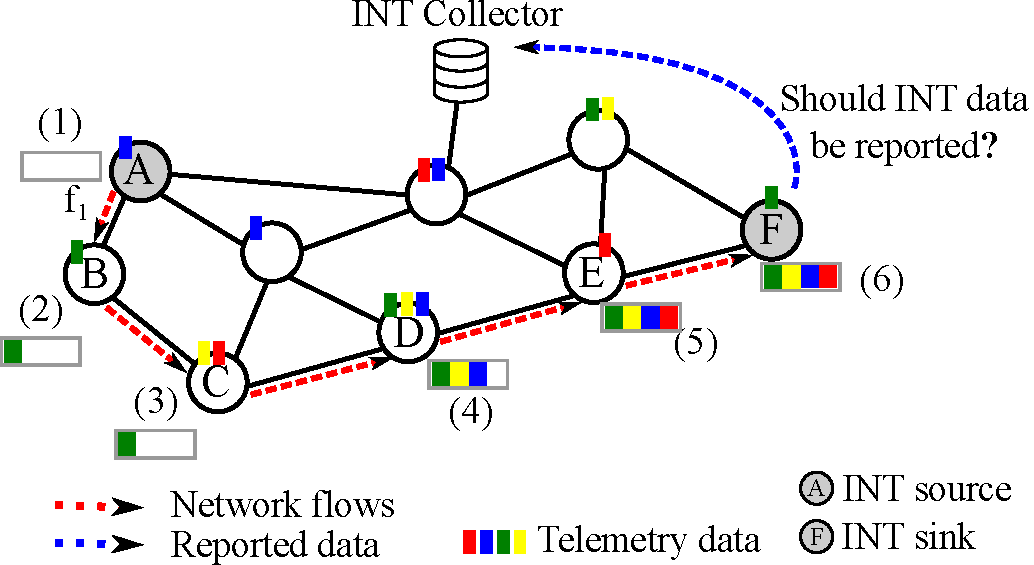
\includegraphics[scale=0.4]{aina-img/telemetry-canofre-aina.pdf}
        \caption{Overview of the problem.}
        \label{fig-problem-overview}
\end{figure}

To fill in this gap, in this work we propose a selective INT report mechanism entirely implemented using a SmartNIC. As previously reported by~\cite{aina2021}, programmable devices have stringent constraints in terms of processing capabilities (e.g., lack of floating-point operations) and memory usage limitations. We assume that the INT sink node is on top of a SmartNIC and, therefore, the decision whether report telemetry data or not is upon the NIC. Our proposed mechanism utilizes a lightweight Exponentially Weighted Moving Average inside the data plane. For that, we implemented it using P4 language and Micro-C routines to allow more complex operations inside the data plane. By performing an extensive performance evaluation using SmartNICs, we show that our proposed approach can reduce the amount of non-important telemetry data sent to INT collector by up to 16X (when compared to the Classical INT), while introducing negligible overhead in terms of packet latency.

The main contributions of this paper can be summarized as:

\begin{itemize}
    \item an in-network mechanism implemented in state-of-the-art SmartNICs to wisely decide when to report INT metadata;
    \item a discussion of current limitations on implementing in-network computing in SmartNIC architectures; and
    \item an open-source code in order to foster reproducibility. 
\end{itemize}

The remainder of this paper is organized as follows. In Section~2, we describe the SmartNIC architecture used in this work. In Section 3, we introduce our proposed approach. In Section 4, we discuss the obtained results. In Section~5, we overview the recent literature regarding in-band network telemetry, and. Last, in Section~6, we conclude this paper with final remarks.


%Due to the rich spectrum of benefits behind INT, there is increasing attention from the networking ecosystem fostered  by the rapid adoption of programmable data planes and domain-specific networking description languages (e.g., P4~\cite{p4-ref}).



%Since its inception, INT has been successfully applied to a series of use cases, including the identification of short-lived network behaviors and network anomalies. 
%Due to the rich spectrum of benefits behind INT, there is increasing attention from the networking ecosystem fostered  by the rapid adoption of programmable data planes and domain-specific networking description languages (e.g., P4~\cite{p4-ref}).
%In short, INT consists of instrumenting the collection of low-level network monitoring statistics directly from the data plane. Probing packets consists of specially crafted packets that instruct programmable forwarding devices to collect telemetry data. Figure~1 illustrates the entire INT process. In the first step, probing packets are generated aiming at instrumenting the collection of telemetry data along a given path. For example, the red flow (i.e. $f_1$) -- that is routed through the forwarding devices $A$, $E$, $F$, $G$, $H$, and $I$ -- carries instructions to collect telemetry data from devices $A$ to $H$. In the second step, the collected telemetry data is extracted and reported to an INT collector. 
%In short, INT consists of instrumenting the collection of low-level network statistics directly from the data plane. In the classic hop-by-hop INT (a.k.a INT-MD (eMbed Data)\footnote{INT specification: \url{https://github.com/p4lang/p4-applications/blob/master/docs/INT_v2_1.pdf}}), an INT source node embeds instructions into  production network packets. Then, INT transit nodes embed metadata while an INT sink node strips the instruction out of the packet and sends the accumulated telemetry data to an INT collector.


%\textbf{OLD from here!}


%context
%Programmable Data Planes (PDP) is a mainstream technology that has been recently redesigning the networking domain. PDP allows to (re)define the behavior of network devices (e.g., programmable routers and SmartNICs), allowing to deliver specialized packet processing mechanisms~\cite{p4-ref}. Recent advances in data plane programmability have enabled offloading typical control plane applications to the data plane (e.g., machine learning algorithms~\cite{xiong2019switches}, routing~\cite{8737398-infocom}, or network monitoring~\cite{9330755, 8865384, aina2020-rumenigue}). On shifting the operation of these applications to the data plane, it brings the benefit to process every single packet and react to network conditions in the order of nanoseconds, with minimum control plane intervention.
%
%Despite that, data plane operation might become complex -- and the complexity comes at a price: \emph{lower throughput and higher latency}. 


%Current SmartNIC architectures (e.g., \cite{netronomeArc}) do not limit the number of operations performed by the data plane in a single pipeline stage. For example, a PDP application could trigger the read and write of an unbounded number of registers in a given stage of the packet processing pipeline. Yet, the same application could recirculate the ingress packet multiple times to mimic a loop-based mechanism. These are straightforward examples of simple operations commonly used by more complex PDP applications (e.g., in-network clustering~\cite{xiong2019switches}). Therefore, understanding the current performance limitations of existing SmartNICs is paramount to the design of efficient PDP applications.


%evaluate  different  P4  constructs  and  their  impact  onthe packet processing latency. They gradually increase the complexity of aSmartNIC  pipeline  (i.e.,  including  parser,  control  blocks,  and  deparser)  toidentify the most influential variables and present a generalized estimation

%A recent study~\cite{harkous2019towards} has made the first effort to understand the existing limitations of SmartNICs. Harkous et al.~\cite{harkous2019towards} have focused on evaluating the performance of general PDP metrics such as parsers, control blocks, and header modifications in P4 programs. Despite this effort, no study has yet thoroughly evaluated key building blocks of complex P4 programs (e.g., registers, cryptography functions, or packet recirculation) -- which are essential for most recent P4 applications.
%
%To fill in this gap, we perform an extensive performance evaluation of SmartNICs to understand and quantify PDP application primitives and existing limitations. We focus our evaluation on measuring the performance in terms of latency and throughput for a variety of packet sizes (from 64B to 1500B) when (i) operating multiple registers of different sizes/widths (e.g., used to implement bloom filter alike structures~\cite{hhh-sigcomm}), (ii) matching on multiple tables in the ingress and egress pipeline (e.g., used to implement machine-learning algorithms~\cite{xiong2019switches}), (iii) performing packet recirculation (e.g., used to implement IoT data desegregation~\cite{WANG201998}), and (iv) using cryptography functions and arithmetic operations. Results show that network throughput can degrade up to 8X, while latency can increase as much as 80X when performing memory-intensive operations in the data plane. The main contributions of this paper can be summarized as:

%\begin{itemize}
%    \item an in-depth performance evaluation of SmartNICs;
%    \item a discussion of current limitations in SmartNIC architectures; and
%    \item an open-source code of all experiments in order to foster reproducibility. 
%\end{itemize}

%The remainder of this paper is organized as follows. In Section~2, we describe the SmartNIC architecture used in this work. In Section~3, we overview the recent literature regarding PDP applications and performance evaluation. In Section 4, we present and discuss the obtained results and, in Section~5, we conclude this paper with final remarks. 
